\documentclass[11pt,a4paper]{article}

\usepackage[utf8]{inputenc}
\usepackage[T1]{fontenc}
\usepackage[english]{babel}
\usepackage[a4paper,margin=2.4cm]{geometry}

\usepackage{amsmath, amssymb, amsthm}
\usepackage{mathtools}
\usepackage{stmaryrd}
\usepackage{booktabs}
\usepackage{tabularx}
\usepackage{array}
\usepackage{caption}
\usepackage{subcaption}
\usepackage{float}
\usepackage{enumitem}
\usepackage{microtype}
\usepackage{xcolor}
\usepackage{listings}
\usepackage{fancyhdr}
\usepackage{titlesec}
\usepackage{graphicx}
\usepackage{tikz}
\usetikzlibrary{positioning, arrows.meta, fit, backgrounds, calc, shapes.geometric}
\usepackage[hidelinks]{hyperref}

%  ---  Palette shared with the companion reports  ---
\definecolor{ink}{RGB}{26,30,36}
\definecolor{slate}{RGB}{92,101,112}
\definecolor{mist}{RGB}{233,235,238}
\definecolor{rulegrey}{RGB}{188,194,201}
\definecolor{steel}{RGB}{47,72,102}
\definecolor{steellight}{RGB}{124,146,172}
\definecolor{signal}{RGB}{160,32,45}
\definecolor{southc}{RGB}{51,115,204}
\definecolor{northc}{RGB}{230,128,38}
\definecolor{knows}{RGB}{26,140,70}

\hypersetup{
    colorlinks=true,
    linkcolor=steel,
    citecolor=steel,
    urlcolor=steel,
    pdftitle={The Muddy Children at a Muster Point},
    pdfauthor={Haniel Ulises},
}

\color{ink}

\setlength{\headheight}{22pt}
\pagestyle{fancy}
\fancyhf{}
\fancyhead[L]{\small\textcolor{slate}{\itshape The Muddy Children at a Muster Point}}
\fancyhead[R]{\small\textcolor{slate}{\thepage}}
\renewcommand{\headrulewidth}{0.4pt}
\renewcommand{\headrule}{\hbox to\headwidth{\color{rulegrey}\leaders\hrule height \headrulewidth\hfill}}

\titleformat{\section}{\normalfont\large\bfseries\color{ink}}{\thesection}{0.7em}{}
\titleformat{\subsection}{\normalfont\normalsize\bfseries\color{ink}}{\thesubsection}{0.7em}{}
\titleformat{\paragraph}[runin]{\normalfont\bfseries\color{slate}}{}{0em}{}[.]

\captionsetup{font=small, labelfont={bf,color=slate}, textfont=footnotesize}

\theoremstyle{definition}
\newtheorem{definition}{Definition}
\newtheorem{proposition}{Proposition}
\newtheorem{lemma}{Lemma}
\newtheorem{corollary}{Corollary}
\newtheorem{fact}{Fact}
\newtheorem{remark}{Remark}

\lstdefinestyle{sys}{
    backgroundcolor=\color{mist},
    basicstyle=\ttfamily\scriptsize\color{ink},
    keywordstyle=\color{steel}\bfseries,
    commentstyle=\color{slate}\itshape,
    stringstyle=\color{slate},
    morecomment=[l]{;},
    morekeywords={:types,:predicates,:objects,:agents,:goal,:init,:event,:action,:action-type,:observability-conditions,:precondition,:effects,:events,:relations,:designated,:conditions,:observability-types},
    frame=single,
    rulecolor=\color{rulegrey},
    framesep=5pt,
    xleftmargin=6pt,
    xrightmargin=0pt,
    breaklines=true,
    showstringspaces=false,
    columns=fullflexible,
    captionpos=b,
}
\lstset{style=sys}

%  ---  Notation  ---
\newcommand{\Ag}{\mathcal{A}}
\newcommand{\Mod}{\mathcal{M}}
\newcommand{\Ev}{\mathcal{E}}
\newcommand{\prd}{\otimes}
\newcommand{\Kop}[1]{K_{#1}}
\newcommand{\Eop}[1]{E_{#1}}
\newcommand{\Cop}[1]{C_{#1}}
\newcommand{\Kw}[1]{\mathit{Kw}_{#1}}
\newcommand{\code}[1]{\texttt{\small #1}}
\newcommand{\ag}[1]{\mathit{#1}}
\newcommand{\job}{\mathit{job}}
\newcommand{\pre}{\mathit{pre}}
\newcommand{\post}{\mathit{post}}
\newcommand{\dist}{\mathrm{dist}}
\newcommand{\depth}{\mathrm{depth}}
\newcommand{\atview}{\mathit{at\text{-}view}}
\newcommand{\sem}[1]{\llbracket #1 \rrbracket}

\newcommand{\faulty}{\mathit{faulty}}
\newcommand{\Hc}{\mathcal{H}}
\newcommand{\some}{\theta}
\newcommand{\one}{\mathbf{1}}
\newcommand{\zero}{\mathbf{0}}

\begin{document}

\begin{titlepage}
\centering
\vspace*{2.4cm}
{\color{rulegrey}\rule{\textwidth}{0.8pt}}\\[0.9cm]
{\LARGE\bfseries The Muddy Children at a Muster Point\par}
\vspace{0.5cm}
{\large\color{slate} Common Knowledge from the Public Announcement\\
of a Fact Every Robot Already Knows\par}
\vspace{0.7cm}
{\color{rulegrey}\rule{\textwidth}{0.8pt}}\\[1.4cm]

{\large Haniel Ulises\par}
\vspace{0.3cm}
{\color{slate} Epistemic Robotics}\\
\vspace{0.15cm}
{\color{slate}\today}

\vfill
{\color{slate}\small
At the end of a shift $N$ robots meet at a muster point. Each carries a status
lamp, lit when its calibration has drifted, which every other robot can see and
it cannot. A supervisor says over the public address that at least one of them
is faulty; then a bell rings, and at each ring every robot that knows it is
faulty leaves for the calibration bay. This is the muddy children puzzle,
stated as an epistemic planning task whose goal is that every robot knows
whether it is faulty.

\vspace{0.6em}
With $k \geq 2$ lamps lit the announcement tells no robot anything it did not
know: each sees a lit lamp. What it changes is the depth of the group's
knowledge of that fact, from $E^{k-1}$ to common knowledge. We prove that
without the announcement no robot ever learns its own lamp, so that every bell
leaves the model as it was and no policy exists at any depth; that with it the
$k$ faulty robots know after $k-1$ silent bells and leave at the $k$-th, at
which the others learn that they are not faulty; and that a policy of depth
$N$ exists and none of smaller depth. Aletheia agrees for two to ten robots: a
policy of depth $N$ with $N$ leaves, found in $3N(N+1)/2$ expansions, and no
policy without the public address, which its relaxation proves. The report is
the counterpart of the coordinated attack, where common knowledge was a
precondition no private message could supply; here a public event supplies it,
and that is what makes the bells informative. Four robots were run on both
floors in Gazebo through ePlanSys: with the announcement the three faulty robots
left at the third bell and the fourth went back to work; without it four bells
passed and nobody moved.}
\vspace{1.2cm}
\end{titlepage}

\tableofcontents
\newpage

%  ======================================================================
\section{Scope}
\label{sec:scope}

The companion report on the coordinated attack~\cite{ulises2026ca} states
common knowledge as the precondition of a joint action, proves that a lossy
radio cannot supply it, and shows a public signal supplying it in one update.
This report takes a problem in which common knowledge is not a precondition
stated in the domain, and is still what an epistemic policy turns on: the
muddy children~\cite{littlewood1953, mdh1986, fhmv1995}, in the form of robots
at a muster point with status lamps they cannot see on themselves.

Four claims are advanced.

\begin{enumerate}[leftmargin=1.4em, itemsep=2pt]
  \item Before the announcement, at a world with $k$ lamps lit, ``some lamp is
        lit'' holds at depth exactly $E^{k-1}$ (Lemma~\ref{lem:hdepth}); every
        robot knows it as soon as $k \geq 2$, and it is common knowledge only
        after the announcement.
  \item Without the announcement no robot ever learns its own lamp: every bell
        is the identity update, and no policy exists, of any depth
        (Proposition~\ref{prop:silent}).
  \item With it, $k$ faulty robots know after $k-1$ silent bells and leave at
        the $k$-th, at which the others learn that they are not faulty
        (Proposition~\ref{prop:bells}); a policy of depth $N$ with $N$ leaves
        exists, and none of smaller depth (Proposition~\ref{prop:depth}).
  \item The planner agrees, for two to ten robots, on both floors, and both
        floors were executed with four robots in Gazebo through ePlanSys, the
        bell's outcome given by the robots that know at the actual world
        (Section~\ref{sec:runs}).
\end{enumerate}

Three bounds are stated at the outset. The lamps are the fleet's diagnostics,
and the robots' observation of each other's lamps is a modelling assumption,
checked on the floor plan as a line of sight between every pair of places on
the muster ring and not perceived by a camera. The bell observes whether any
robot left, not which robots did; Section~\ref{sec:bells} shows that the model
needs no more. And the robots do not reason for themselves: which of them know
they are faulty is read, at each bell, from the model the epistemic state
maintains, evaluated at the world the lamps make actual.

%  ======================================================================
\section{Preliminaries}
\label{sec:prelim}

The definitions are those of the companion report: epistemic models
$\Mod = (W, R, V, W_d)$, the group modalities $\Eop{G}$ and $\Cop{G}$ over
$R_G = \bigcup_{a \in G} R_a$, and event models with observability types and
their product update. We recall the two facts used below.

\begin{definition}[Distance and depth]
For $\Mod, w \models \varphi$, $\dist_w(\varphi)$ is the length of the shortest
$R_G$-path from $w$ to a world where $\varphi$ fails, and $\infty$ if there is
none; $\depth_w(\varphi) = \dist_w(\varphi) - 1$.
\end{definition}

\begin{lemma}[\cite{ulises2026ca}]
\label{lem:depth}
If $\Mod$ is $\mathrm{S5}$ and $\Mod, w \models \varphi$, then for $k \geq 1$,
$\Mod, w \models \Eop{G}^k\varphi$ iff $k \leq \depth_w(\varphi)$, and
$\Mod, w \models \Cop{G}\varphi$ iff $\dist_w(\varphi) = \infty$.
\end{lemma}

\begin{definition}[Public sensing]
For a formula $\psi$, $P(\psi)$ has events $e^+$ with $\pre(e^+) = \psi$ and
$e^-$ with $\pre(e^-) = \neg\psi$, trivial postconditions, both designated, and
$Q(\tau) = \{(e^+,e^+), (e^-,e^-)\}$ for every agent.
\end{definition}

\begin{lemma}[Public sensing restricts]
\label{lem:restrict}
Let $(w,e) \in \Mod \prd P(\psi)$. The worlds of $\Mod \prd P(\psi)$ reachable
from $(w,e)$, with their relations and valuations, are those of the
restriction of $\Mod$ to $\{v : \Mod, v \models \pre(e)\}$ reachable from $w$.
\end{lemma}

\begin{proof}
$(v,f) \mathrel{R'_a} (u,g)$ iff $v R_a u$ and $f = g$, so every world reachable
from $(w,e)$ has the event $e$, and $(u,e)$ exists iff $\Mod, u \models
\pre(e)$. The postconditions are trivial.
\end{proof}

\noindent
Both actions of the domain are of this form. The announcement is $P(\some)$
with $\some = \bigvee_i \faulty(i)$, ``some lamp is lit'', and its event $e^-$
can occur only at the world with no lamp lit, which is never designated. The
bell is $P(\lambda)$ with $\lambda = \bigvee_i \Kop{i}\faulty(i)$, ``some robot
knows that it is faulty'': $e^+$ is \code{e-leave} and $e^-$ is \code{e-stay}.

%  ======================================================================
\section{The domain}
\label{sec:domain}

\code{tools/muster.py} writes the domain for $N$ robots $r_1, \dots, r_N$ and
two floors that differ in one line, whether the hall has a public address,
$\mathit{pa}$. The atom $\faulty(i)$ says that $r_i$'s calibration has drifted
and its lamp is lit. Every robot sees every other robot's lamp and not its own,
and that is common knowledge; that some lamp is lit is true, and not common
knowledge. The goal is that every robot knows whether it is faulty:
\[
  \gamma \;=\; \bigwedge_{i} \Kw{r_i}\,\faulty(i).
\]

\begin{table}[H]
\centering\small
\caption{The actions of the domain.}
\label{tab:actions}
\begin{tabularx}{\textwidth}{@{}>{\raggedright\arraybackslash}p{2.6cm} >{\raggedright\arraybackslash}p{3.4cm} >{\raggedright\arraybackslash}X >{\raggedright\arraybackslash}p{2.2cm}@{}}
\toprule
action & type & events & observers \\
\midrule
$\mathit{announce}$ & public announcement & $\mathit{pa} \wedge \some$; $\mathit{pa} \wedge \neg\some$ & everyone \\
$\mathit{bell}$ & public sensing & \code{e-leave}: $\bigvee_i \Kop{i}\faulty(i)$; \code{e-stay}: $\bigwedge_i \neg\Kop{i}\faulty(i)$ & everyone \\
\bottomrule
\end{tabularx}
\end{table}

\begin{lstlisting}[caption={The bell, in the domain \code{tools/muster.py} writes.}, label={lst:bell}]
(:event e-leave
  :parameters (?h - hall)
  :precondition (exists (?i - agent) ([?i] (faulty ?i))))

(:event e-stay
  :parameters (?h - hall)
  :precondition (forall (?i - agent) (not ([?i] (faulty ?i)))))

(:action bell
  :parameters (?h - hall)
  :action-type (public-sensing (e-leave ?h) (e-stay ?h))
  :observability-conditions (default Fully))
\end{lstlisting}

\paragraph{Why the bell observes only whether anyone left} On the floor every
robot sees which robots drive off. The model takes less, a public sensing of
$\lambda$, and Section~\ref{sec:bells} shows that it loses nothing: after the
first departure every robot already knows whether it is faulty, so who left
adds no information the goal needs.

\paragraph{Why the hall is a parameter} plank grounds an action once for each
assignment of its parameters, and an action with none is never grounded. Both
actions take the hall, of which each problem has one, \code{muster}.

%  ======================================================================
\section{The model}
\label{sec:model}

\begin{definition}[The muster model]
$\Hc_N = (W, R, V, W_d)$ with $W = \{0,1\}^N$, $u R_i v$ iff $u_j = v_j$ for every
$j \neq i$, $V(u) = \{\faulty(i) : u_i = 1\} \cup V_{\mathit{pa}}$, and
$W_d = W \setminus \{\zero\}$. For $u \in W$ let $|u|$ be the number of lamps
lit, and $u^{i}$ the world that differs from $u$ in the $i$-th lamp only.
\end{definition}

\noindent
$R_i$ relates two worlds exactly when they differ at most in $r_i$'s own lamp,
which is the statement that $r_i$ sees every lamp but its own. Each $R_i$ is an
equivalence with classes $\{u, u^i\}$, and $\Hc_N$ is $\mathrm{S5}$. plank
grounds the initial model of the problem to $\Hc_N$: $2^N$ worlds, of which
$2^N - 1$ designated. The designated worlds are the planner's uncertainty about
the lamps, not any robot's; what a robot knows is what it knows at the actual
world, the one whose lit lamps are the faults.

\begin{lemma}[The depth before the announcement]
\label{lem:hdepth}
For $u \in W_d$ with $|u| = k$, $\dist_u(\some) = k$ in $\Hc_N$: the robots have
$\Eop{G}^{k-1}\some$ at $u$ and not $\Eop{G}^{k}\some$.
\end{lemma}

\begin{proof}
$\some$ fails only at $\zero$. An $R_G$-step changes at most one lamp, so a path
from $u$ to $\zero$ has at least $k$ steps; turning the $k$ lit lamps off one at
a time, each step by the robot whose lamp it is, is such a path of $k$ steps.
Lemma~\ref{lem:depth} gives the rest.
\end{proof}

\noindent
With $k = 1$ the faulty robot does not know that any lamp is lit, since it sees
none. With $k \geq 2$ every robot knows it, and the depth $E^{k-1}$ falls short
of common knowledge by a chain through the faulty robots: $r_1$ considers that
only $r_2, \dots, r_k$ are lit, in which world $r_2$ considers that only
$r_3, \dots, r_k$ are, and so on down to the world with no lamp lit.

%  ======================================================================
\section{Silence}
\label{sec:silent}

\begin{proposition}[Without the announcement, no robot learns its lamp]
\label{prop:silent}
In $\Hc_N$ no robot knows whether it is faulty, at any world:
$\Hc_N, u \not\models \Kop{i}\faulty(i)$ and
$\Hc_N, u \not\models \Kop{i}\neg\faulty(i)$ for every $u$ and $i$. Hence the
bell's \code{e-leave} occurs nowhere, \code{e-stay} occurs everywhere, and the
part of $\Hc_N \prd \mathit{bell}$ reachable from any world is $\Hc_N$ again.
\end{proposition}

\begin{proof}
$u R_i u^i$, and $u$ and $u^i$ disagree on $\faulty(i)$. So $\lambda$ fails at
every world, and by Lemma~\ref{lem:restrict} the \code{e-stay} copy of $\Hc_N$
is $\Hc_N$, restricted to all of $W$.
\end{proof}

\begin{corollary}[No policy without the public address]
\label{cor:silent}
On the floor without a public address no sequence of actions makes $\gamma$
hold, and no policy exists, of any depth.
\end{corollary}

\begin{proof}
$\mathit{announce}$ requires $\mathit{pa}$, which is false, so every execution
is a sequence of bells. By Proposition~\ref{prop:silent} and induction each
leaves the model $\Hc_N$, at which $\gamma$ fails at every world.
\end{proof}

\noindent
Every robot can see, at a world with three lamps lit, that some lamp is lit,
and the bell still teaches nothing. The reason is the chain of
Lemma~\ref{lem:hdepth}: that nobody left is what every robot expected in every
world it considers possible, including the world with no lamp lit at the end of
the chain, where nobody could have left.

%  ======================================================================
\section{The announcement and the bells}
\label{sec:bells}

For $0 \leq j < N$ let $\Mod_j$ be $\Hc_N$ restricted to
$\{u : |u| \geq j + 1\}$, and $L_j$ be $\Hc_N$ restricted to
$\{u : |u| = j\}$.

\begin{lemma}[The announcement]
\label{lem:announce}
The part of $\Hc_N \prd \mathit{announce}$ reachable from a designated world is
$\Mod_0$, and $\Mod_0 \models \Cop{G}\some$.
\end{lemma}

\begin{proof}
At a designated world the event that occurs is the one with $\some$, and by
Lemma~\ref{lem:restrict} the reachable part is $\Hc_N$ restricted to the worlds
with a lamp lit, that is $\Mod_0$. $\some$ holds at all of them, so its distance
is infinite.
\end{proof}

\begin{proposition}[The bells after the announcement]
\label{prop:bells}
In $\Mod_j$, at $u$:
\begin{enumerate}[leftmargin=1.6em, itemsep=1pt]
  \item $r_i$ knows that it is faulty iff $u_i = 1$ and $|u| = j+1$, and no robot
        knows that it is not faulty;
  \item the bell gives \code{e-leave} iff $|u| = j+1$, and then the reachable
        part of the update is $L_{j+1}$, in which every robot knows whether it
        is faulty; otherwise it gives \code{e-stay}, and the reachable part is
        $\Mod_{j+1}$.
\end{enumerate}
\end{proposition}

\begin{proof}
In $\Mod_j$ the class of $u$ for $r_i$ is $\{u, u^i\}$ if $|u^i| \geq j+1$, and
$\{u\}$ otherwise. If $u_i = 0$ then $|u^i| = |u| + 1$, so $u^i$ is present, and
$r_i$ does not know its lamp. If $u_i = 1$ then $|u^i| = |u| - 1$, which is
below $j+1$ exactly when $|u| = j+1$; then $r_i$'s class is $\{u\}$ and it knows
that it is faulty. This is the first part. So $\lambda$ holds at $u$ iff
$|u| = j+1$, and by Lemma~\ref{lem:restrict} the \code{e-leave} part is
$\Mod_j$ restricted to $|u| = j+1$, which is $L_{j+1}$, and the \code{e-stay}
part is $\Mod_j$ restricted to $|u| \geq j+2$, which is $\Mod_{j+1}$. In
$L_{j+1}$ two distinct worlds have the same number of lamps lit and so differ in
at least two, and no relation joins them: every class is a single world, and
every robot knows its lamp.
\end{proof}

\begin{corollary}[$k$ faulty robots]
\label{cor:k}
At a world with $k$ lamps lit, after the announcement the first $k-1$ bells
give \code{e-stay}. After the $(k-1)$-th the $k$ faulty robots know that they
are faulty; the $k$-th gives \code{e-leave}, and after it the others know that
they are not. With $k = N$, $\Mod_{N-1}$ is the single world $\one$, and every
robot knows after $N - 1$ bells.
\end{corollary}

\begin{proposition}[The depth of a policy]
\label{prop:depth}
On the floor with a public address the policy that announces, and then rings
the bell until it gives \code{e-leave} or has rung $N-1$ times, satisfies
$\gamma$ at every leaf; it has depth $N$ and $N$ leaves. No policy of smaller
depth exists.
\end{proposition}

\begin{proof}
By Corollary~\ref{cor:k}, the branch on which the $j$-th bell first gives
\code{e-leave}, for $j \leq N-1$, ends in $L_j$, and the branch of $N-1$
\code{e-stay} ends in $\Mod_{N-1} = \{\one\}$; $\gamma$ holds at every world of
each. That is $N$ leaves, and the longest branch has $1 + (N-1)$ actions. For
the lower bound take the designated world $\one$. Bells before the
announcement leave the model unchanged (Proposition~\ref{prop:silent}), so the
branch a policy follows at $\one$ must announce, and after the announcement and
$j$ bells, all of which give \code{e-stay} at $\one$ while $j \leq N-1$, the
model is $\Mod_j$. For $j < N-1$, $r_i$ considers $\one^i$, with $N-1 \geq j+1$
lamps lit, so it does not know its lamp at $\one$ and $\gamma$ fails there.
The branch therefore has at least $1 + (N-1)$ actions.
\end{proof}

\noindent
With $k \geq 2$ the announcement gives no robot a fact it lacked, and
Proposition~\ref{prop:silent} shows that the bells alone give nothing. What the
announcement gives is the depth: it turns $E^{k-1}\some$ into $C\some$. The
first silent bell is then informative, because after the announcement a world
with one lamp lit is one in which that robot knows it is faulty and leaves, so
that nobody leaving rules every such world out.

%  ======================================================================
\section{Planning results}
\label{sec:planning}

Both floors were grounded by plank and solved by Aletheia with AO$^*$ at one
thread, for two to ten robots. On the floor without a public address
Aletheia's knowledge relaxation proves the goal unreachable before any search,
which Corollary~\ref{cor:silent} confirms. On the floor with one it returns
the policy of Proposition~\ref{prop:depth}, of depth $N$ with $N$ leaves; the
trace tool replays the policy for four robots and reports $\gamma$ at every
designated world of each of the four leaves, covering the fifteen patterns with
a lamp lit.

\begin{table}[H]
\centering\small
\caption{Both floors for $N$ robots. Times are wall-clock for the planner
process, loading included.}
\label{tab:planning}
\begin{tabular}{@{}r r r r r r r r@{}}
\toprule
& & \multicolumn{4}{c}{public address} & \multicolumn{2}{c}{none} \\
\cmidrule(lr){3-6}\cmidrule(l){7-8}
$N$ & worlds & depth & leaves & expansions & time & result & time \\
\midrule
2 & 4 & 2 & 2 & 9 & 0.003\,s & unreachable & 0.003\,s \\
3 & 8 & 3 & 3 & 18 & 0.003\,s & unreachable & 0.003\,s \\
4 & 16 & 4 & 4 & 30 & 0.004\,s & unreachable & 0.003\,s \\
5 & 32 & 5 & 5 & 45 & 0.006\,s & unreachable & 0.004\,s \\
6 & 64 & 6 & 6 & 63 & 0.012\,s & unreachable & 0.004\,s \\
7 & 128 & 7 & 7 & 84 & 0.031\,s & unreachable & 0.007\,s \\
8 & 256 & 8 & 8 & 108 & 0.071\,s & unreachable & 0.007\,s \\
9 & 512 & 9 & 9 & 135 & 0.239\,s & unreachable & 0.014\,s \\
10 & 1\,024 & 10 & 10 & 165 & 0.690\,s & unreachable & 0.023\,s \\
\bottomrule
\end{tabular}
\end{table}

\noindent
The expansions are $3N(N+1)/2$ for every $N$ measured; that is an observation,
not a property proved here. The time grows with the model, which doubles with
each robot, and not with the search, which grows quadratically.

%  ======================================================================
\section{Four robots, three lamps lit}
\label{sec:trace}

Table~\ref{tab:trace} follows the actual world with $r_1$, $r_2$ and $r_3$ lit,
on both floors, as the trace tool computes it from the task plank grounds.

\begin{table}[H]
\centering\small
\caption{Four robots with $r_1$, $r_2$ and $r_3$ lit. Worlds are those
reachable from the actual world; a robot is marked when it knows its lamp.}
\label{tab:trace}
\begin{tabular}{@{}l l r l l@{}}
\toprule
floor & action & $|W|$ & knows its lamp & depth of $\some$ \\
\midrule
public address & initial & 16 & none & $E^2$ \\
 & $\mathit{announce}$ & 15 & none & $C$ \\
 & $\mathit{bell}$ $\to$ \code{e-stay} & 11 & none & $C$ \\
 & $\mathit{bell}$ $\to$ \code{e-stay} & 5 & $r_1, r_2, r_3$: faulty & $C$ \\
 & $\mathit{bell}$ $\to$ \code{e-leave} & 1 & all; $r_4$: not faulty & $C$ \\
\midrule
none & initial & 16 & none & $E^2$ \\
 & $\mathit{bell}$ $\to$ \code{e-stay}, four times & 16 & none & $E^2$ \\
\bottomrule
\end{tabular}
\end{table}

\noindent
The counts are those of Section~\ref{sec:bells}: $\Mod_0$ has $2^4 - 1 = 15$
worlds, $\Mod_1$ the eleven with two or more lamps lit, $\Mod_2$ the five with
three or four, and $L_3$ has four worlds, none related to another, so that one
is reachable. Before the announcement the chain that blocks common knowledge
runs through the three faulty robots, as Lemma~\ref{lem:hdepth} describes. With
only $r_2$ lit, $r_2$ knows that it is faulty from the announcement alone, and
the first bell gives \code{e-leave}.

%  ======================================================================
\section{The floor}
\label{sec:floor}

The floor is the AWS RoboMaker small warehouse, the world of the robot-warehouse
demonstrations, unchanged, with a muster point, a calibration bay and a public
address added on its open floor (Figure~\ref{fig:floor}). The floor plan is
rasterised from the world's own collision meshes at 5\,cm. The muster point is
the largest open circle on the floor, with 3.6\,m of clearance; the robots stand
on a ring of 1.2\,m about its centre, facing in. The calibration bay is in the
room at the north-west corner, and each robot's station, where it starts and
returns to, is at the end of the west or the middle corridor.

\begin{figure}[H]
\centering
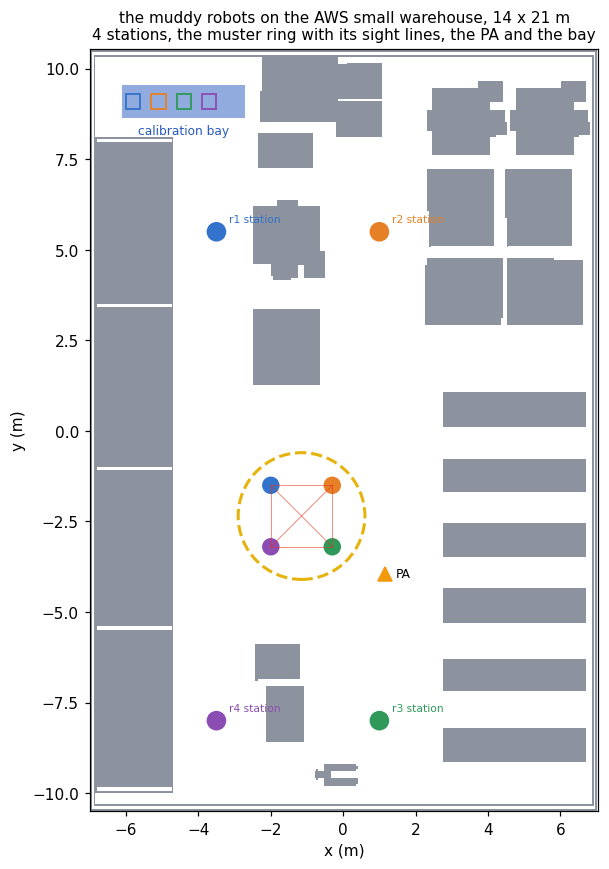
\includegraphics[width=0.55\textwidth]{figures/muddy_robots_floor.png}
\caption{The floor plan with four robots: their stations, the muster ring with
the sight lines between every pair of places on it, the public address, and the
calibration bay with a place for each robot.}
\label{fig:floor}
\end{figure}

The domain makes two claims about the floor, and the floor check tests each on
the plan, by casting rays over the occupied cells or flooding the free ones
(Table~\ref{tab:geometry}). It passes for three, four and five robots.

\begin{table}[H]
\centering\small
\caption{The claims about the floor, each checked on the plan.}
\label{tab:geometry}
\begin{tabularx}{\textwidth}{@{}X X@{}}
\toprule
claim & what depends on it \\
\midrule
on the muster ring every robot has every other robot in line of sight & the initial model, in which each robot knows whether every other is faulty \\
every place a robot is sent is reachable from where it is sent from, over the plan inflated by 0.35\,m & a correct policy, and the dismissal after it, are drivable \\
\bottomrule
\end{tabularx}
\end{table}

\noindent
The actions are performed by one node that owns every robot's driver. Before
planning it drives the robots from their stations to the ring. The
announcement lights a lamp on the public-address mast. At the bell the node
waits for the model that includes the previous update, finds the robots that
know they are faulty at the actual world, and refuses if the model says so of
a robot whose lamp is dark, or if no designated world matches the lamps. It
then sends the robots that know to the bay one at a time, nearest first, and
reports \code{e-leave}, or reports \code{e-stay} if there are none. After the
policy every robot is dismissed on what it knows: the faulty to the bay, the
others back to their stations, and the dismissal is refused if the model's
verdict on any robot disagrees with its lamp.

%  ======================================================================
\section{Runs}
\label{sec:runs}

Both floors were run with four robots and $r_1$, $r_2$ and $r_3$ lit, and
recorded on a virtual display with RViz and Gazebo side by side. In the tables
the model column gives the worlds the robots can still consider, those
reachable from the actual world, then the patterns the executor cannot rule
out, the designated worlds, and the depth of ``some lamp is lit'' at the actual
world.

\begin{table}[H]
\centering\small
\caption{The floor with a public address, as the run reported it.}
\label{tab:pa-run}
\begin{tabularx}{\textwidth}{@{}l X r@{}}
\toprule
action & reported & model \\
\midrule
assembly & every robot at its place on the ring after 16 to 25\,s, each in sight of every other robot's lamp & 16 / 15, $E^2$ \\
plan & 4 policy items, 4 leaves, 0.1\,s & \\
$\mathit{announce}$ & ``at least one of you is faulty'', over the public address & 15 / 15, $C$ \\
$\mathit{bell}$ & no robot knows whether it is faulty, and nobody moves: \code{e-stay} & 11 / 11, $C$ \\
$\mathit{bell}$ & nobody moves: \code{e-stay}; $r_1$, $r_2$ and $r_3$ now know that they are faulty & 5 / 5, $C$ \\
$\mathit{bell}$ & $r_1$, $r_2$ and $r_3$ know that they are faulty and leave, one at a time: \code{e-leave}; in the bay after 34, 41 and 48\,s & 1 / 4, $C$ \\
dismissal & $r_4$ knows that it is not faulty and goes back to its station, after 20\,s; the three are in the bay & \\
\bottomrule
\end{tabularx}
\end{table}

\begin{table}[H]
\centering\small
\caption{The floor without a public address, as the run reported it.}
\label{tab:silent-run}
\begin{tabularx}{\textwidth}{@{}l X r@{}}
\toprule
action & reported & model \\
\midrule
assembly & every robot at its place on the ring after 17 to 24\,s & 16 / 15, $E^2$ \\
plan & no policy, after 0.2\,s; the mission rings the bell four times by hand & \\
$\mathit{bell}$, four times & no robot knows whether it is faulty, and nobody moves: \code{e-stay} & 16 / 15, $E^2$ \\
dismissal & no robot knows whether it is faulty, and every robot stays where it is & \\
\bottomrule
\end{tabularx}
\end{table}

\noindent
The counts are those of Table~\ref{tab:trace}, and the designated worlds after
each bell are those of Proposition~\ref{prop:bells}: the fifteen patterns with a
lamp lit, then the eleven with two or more, the five with three or four, and
after \code{e-leave} the four with exactly three, at each of which every robot
knows its lamp. On the floor without a public address the designated worlds
stayed at fifteen through four bells, as Proposition~\ref{prop:silent} says,
and the mission confirmed through the epistemic state that no robot knew
whether it was faulty before it reported that as the expected outcome.

\begin{figure}[H]
\centering
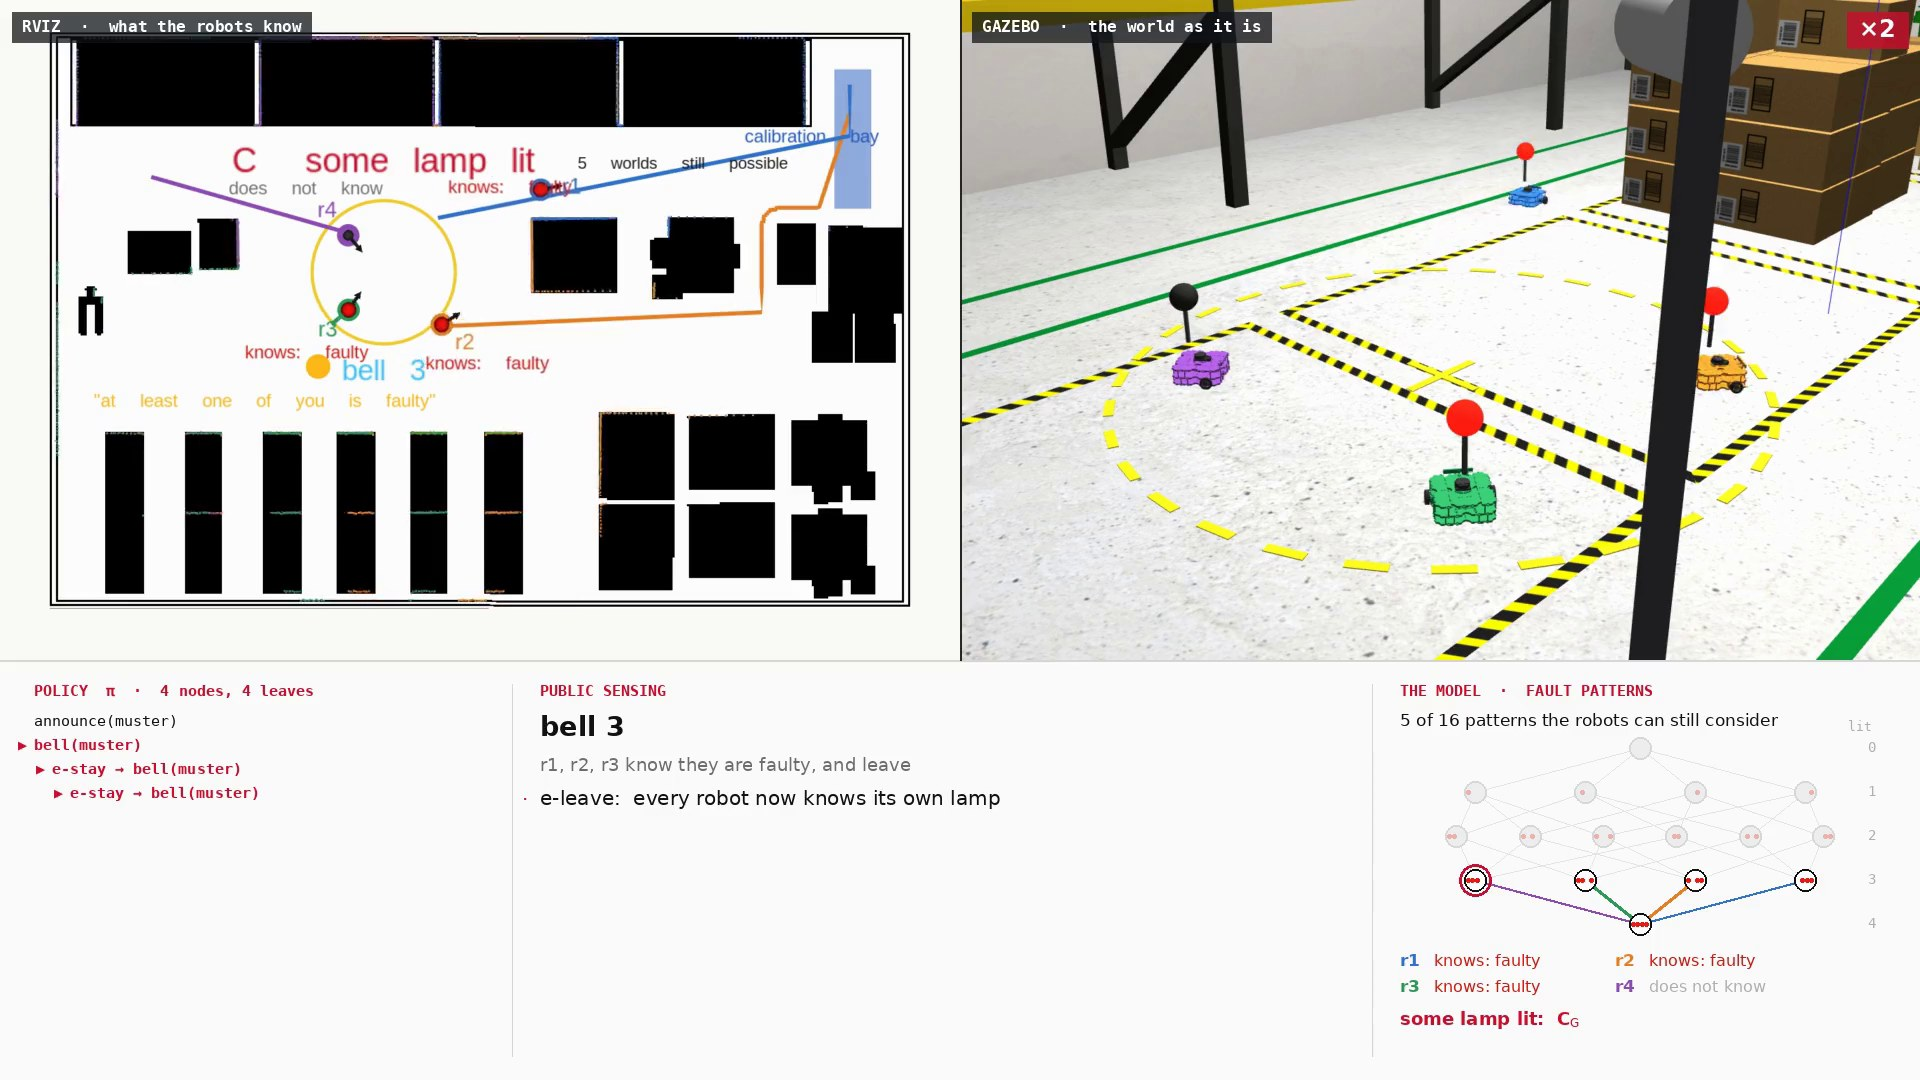
\includegraphics[width=\textwidth]{figures/muddy_robots_frame_bell.jpg}\\[0.4em]
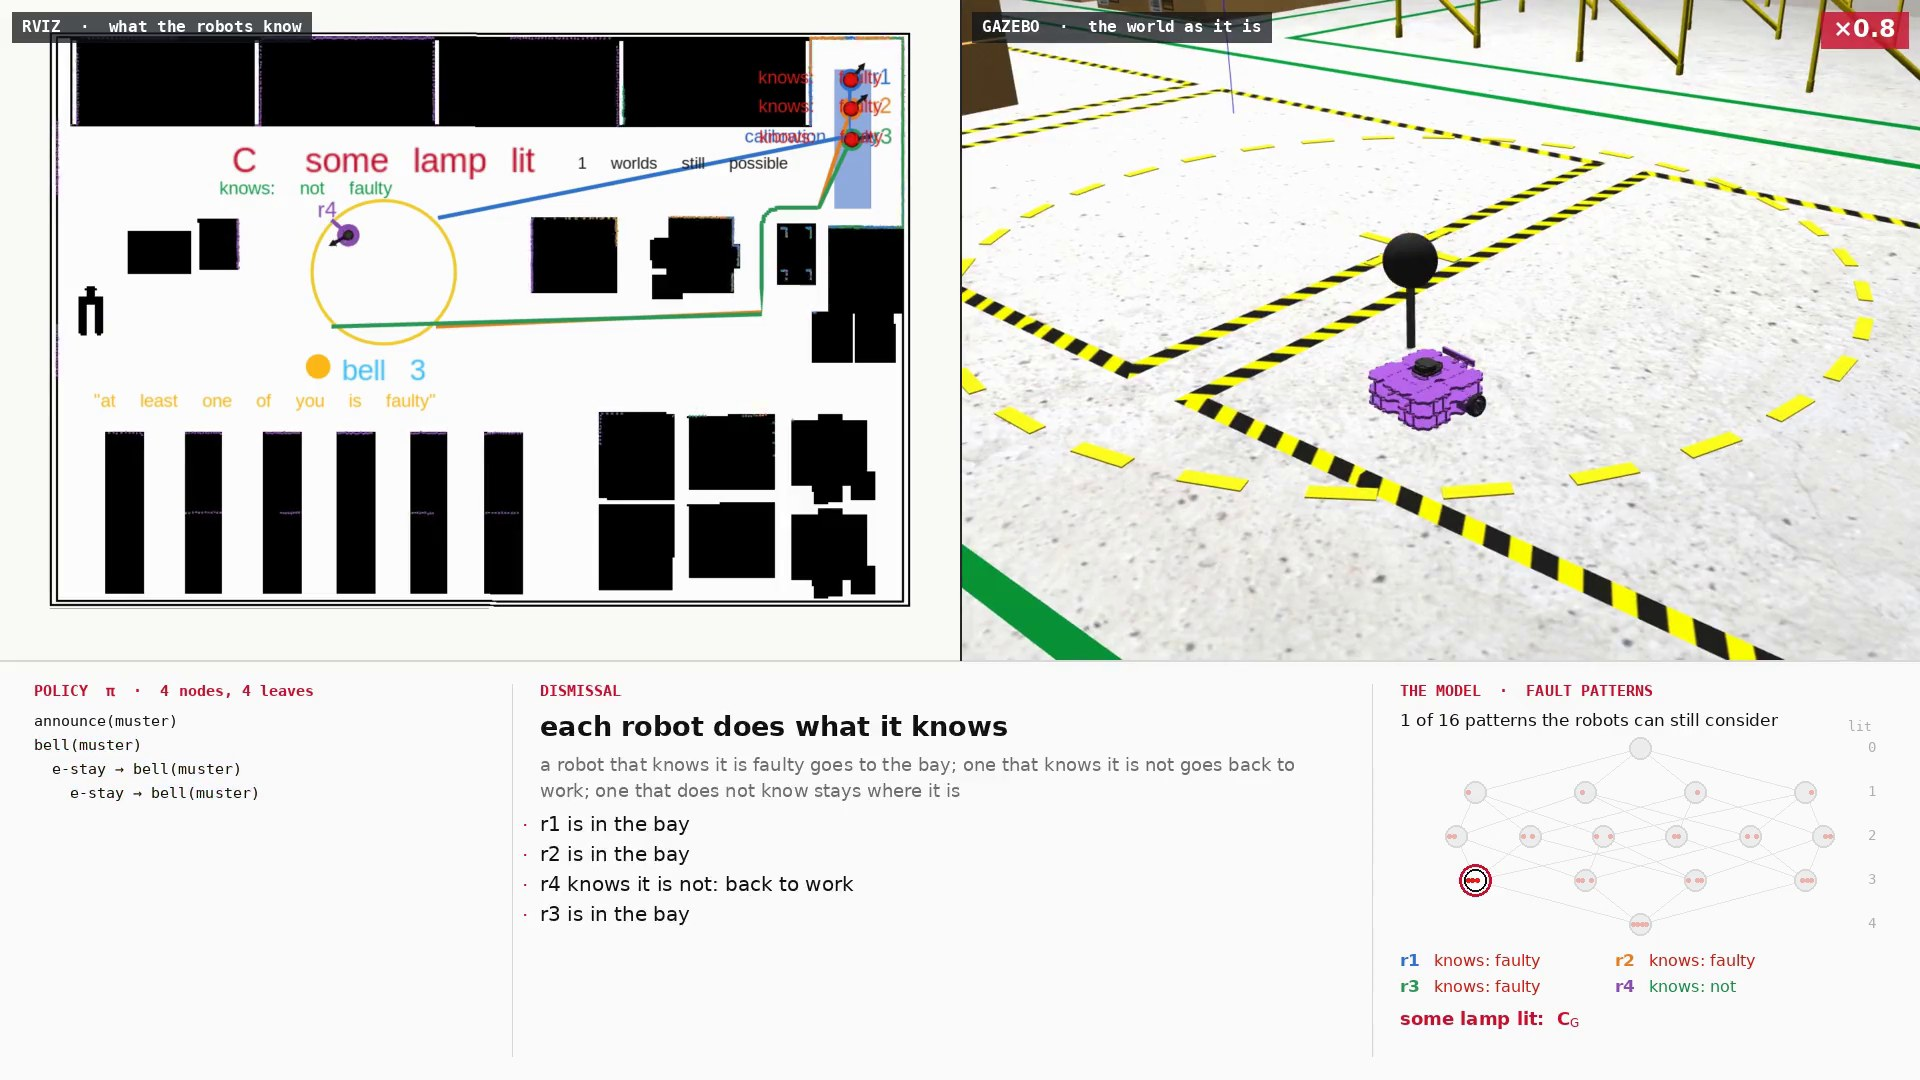
\includegraphics[width=\textwidth]{figures/muddy_robots_frame_dismissal.jpg}
\caption{Two frames of the film. Above, the third bell: $r_1$, $r_2$ and $r_3$
know that they are faulty and leave one at a time, $r_4$ does not know, and
five patterns remain, the four with three lamps lit and the one with four.
Below, the dismissal: one pattern remains for the robots, $r_4$ knows that it is
not faulty and drives back to its station, and the three are in the bay.}
\label{fig:frames}
\end{figure}

%  ======================================================================
\section{Defects}
\label{sec:defects}

\paragraph{Knowledge judged at the designated worlds} The first run took a robot
to know that it was faulty when it did at every designated world, the
fifteen patterns the executor could not rule out, and not at the actual one.
After two silent bells $r_1$ knows that it is faulty at the actual world, where
$r_1$, $r_2$ and $r_3$ are lit, and not at the world where $r_2$, $r_3$ and
$r_4$ are; under that reading no robot knew, and the third bell reported
\code{e-stay}. The epistemic state applies the outcome a performer reports,
and \code{e-stay} removed every world with three lamps lit, the actual world
among them. The model was left with the world in which all four are lit, the
dismissal sent $r_4$, whose lamp was dark, to the bay, and the mission
reported the goal achieved, since in that model every robot knew whether it
was faulty. The designated worlds are the planner's uncertainty about the
lamps and not any robot's. The crew now evaluates knowledge at the actual
world, the bell refuses when no designated world matches the lamps, and the
dismissal refuses when the model and a lamp disagree.

\paragraph{Three robots leaving at once} When the three faulty robots left the
ring together they drove into one another across it: $r_1$ reached the bay
after 30\,s, $r_2$ after 32\,s and $r_3$ after 243\,s. A robot leaving the ring
now steps out along its radius first, and the robots leave one at a time,
nearest the bay first, five seconds apart; in the next run they arrived after
31, 36 and 41\,s.

\paragraph{A goal written as a sentence} On the floor without a public address
the mission rings the bell by hand, since there is no policy, and the policy it
builds for that carried its goal as an English sentence, which the behaviour
tree parsed as a formula. It is now
$\bigwedge_i \Kw{r_i}\,\faulty(i)$, and the executor's report that the goal
does not hold at the end is the expected outcome on that floor.

\paragraph{Guards added on review} The bell refuses when no model has arrived,
and when no state message newer than the end of the previous action arrives
within 10\,s, so that it never reads a model that lacks an update. A formula
check the epistemic state cannot answer fails the mission, where it had been
counted as a robot not knowing; on the floor without a public address that
would have read as the expected outcome.

%  ======================================================================
\section{The counterpart of the coordinated attack}
\label{sec:attack}

In the coordinated attack, common knowledge of the stand is the precondition
of the lift, and the question is which channel can supply it: a lossy message
adds at most one level of mutual knowledge, so no number of them can, and one
public signal seen from common viewpoints does. Here common knowledge is not
asked for by any precondition, and the same distinction decides the outcome. The
robots begin with $E^{k-1}\some$, which a finite exchange of messages could have
raised a level at a time; the bells, public events, teach nothing at that depth
(Proposition~\ref{prop:silent}); and one public announcement, of a fact every
robot already knows, gives $C\some$, after which each public bell removes one
layer of the model.

Halpern and Moses treat both puzzles in their account of common knowledge in
distributed systems~\cite{halpern1990}. The two domains place the public event
differently: at the end of the coordinated attack, where it makes the lift
applicable, and at the start of the muster, where it makes the bells
informative.

%  ======================================================================
\section{Directions for the next iteration}
\label{sec:next}

\paragraph{An announcement over the radio} If the supervisor's message reached
each robot over the lossy channel of the coordinated attack, it would add at
most one level of mutual knowledge to $\some$, and common knowledge would not
arise. Which fault patterns the bells would then settle, as a function of the
depth the message reaches, is a question the domain can put to the planner.

\paragraph{A robot that cannot see one other} If a pillar hides $r_j$'s lamp from
$r_i$, $R_i$ relates worlds that differ in either lamp, the model is no longer
the hypercube, and the number of bells a muster needs depends on the pattern of
occlusion; the floor check would then be a statement about which pairs see
each other and not a requirement that all do.

%  ======================================================================
\begin{thebibliography}{9}
\bibitem{ba2011} T.~Bolander and M.~B. Andersen.
  Epistemic planning for single- and multi-agent systems.
  \emph{Journal of Applied Non-Classical Logics}, 21(1):9--34, 2011.
\bibitem{fhmv1995} R.~Fagin, J.~Y. Halpern, Y.~Moses and M.~Y. Vardi.
  \emph{Reasoning About Knowledge}. MIT Press, 1995.
\bibitem{halpern1990} J.~Y. Halpern and Y.~Moses.
  Knowledge and common knowledge in a distributed environment.
  \emph{Journal of the ACM}, 37(3):549--587, 1990.
\bibitem{littlewood1953} J.~E. Littlewood.
  \emph{A Mathematician's Miscellany}. Methuen, 1953.
\bibitem{mdh1986} Y.~Moses, D.~Dolev and J.~Y. Halpern.
  Cheating husbands and other stories: a case study of knowledge, action, and
  communication. \emph{Distributed Computing}, 1(3):167--176, 1986.
\bibitem{ulises2026ca} H.~Ulises.
  The coordinated attack on a warehouse floor: common knowledge as an action
  precondition, a lossy channel that cannot supply it, and a signal that can.
  Epistemic Robotics report, 2026.
\bibitem{vanditmarsch2007} H.~van Ditmarsch, W.~van der Hoek and B.~Kooi.
  \emph{Dynamic Epistemic Logic}. Springer, 2007.
\end{thebibliography}

%  ======================================================================
\section*{Reproduction}

\begin{lstlisting}
python3 tools/muster.py --robots 4 --out /tmp/muddy           # the domain and both floors
bash tools/validate.sh                                         # seven checks, no simulator
python3 tools/trace.py --task /tmp/muddy_robots_validate/n4/pa/pa-n4.json --faults r1 r2 r3 --bells 4
python3 tools/check_floor.py --robots 4
\end{lstlisting}

\end{document}
